% =================================================================
\documentclass[ 10pt, xcolor = dvipsnames]{beamer}
\usepackage{ beamerthemesplit, lmodern}
\usetheme{Madrid}
\usecolortheme[named=Brown]{structure}
\useinnertheme{rectangles}
\setbeamertemplate{frametitle continuation}{}
\beamertemplatenavigationsymbolsempty
\usepackage{../../macros-general}
\usepackage{../../macros-beamer}
%\graphicspath{{./figures/}}

% =================================================================
\newcommand{\shorttitle}{Blockchain in Industry}
\title[\shorttitle]{Blockchain in Industry}
\author[L. I. Reyes Castro]{Luis I. Reyes Castro}
\institute[BitCapital]{\normalsize Consultor at BitCapital}
\date[Feb-22-2018]{February 22, 2018}

% -----------------------------------------------------------------
\begin{document}
\begin{frame}[noframenumbering]
\titlepage
\end{frame}
\begin{frame}[noframenumbering]
\frametitle{\shorttitle}
\tableofcontents[ subsectionstyle = hide]
\end{frame}

%\AtBeginSection[]
{
\begin{frame}
\frametitle{Contenido del Tema}
\tableofcontents[ currentsection, sectionstyle = show/shaded, subsectionstyle = show/show/hide]
\end{frame}
}
\AtBeginSubsection[]
{
\begin{frame}
\frametitle{Contenido del Tema}
\tableofcontents[ currentsection, currentsubsection, sectionstyle = show/shaded, subsectionstyle = show/shaded/hide]
\end{frame}
}

% Indices
\newcommand{\iava}{$i$\tsup{ava} }
\newcommand{\iavo}{$i$\tsup{avo} }
\newcommand{\java}{$j$\tsup{ava} }
\newcommand{\javo}{$j$\tsup{avo} }
\newcommand{\kava}{$k$\tsup{ava} }
\newcommand{\kavo}{$k$\tsup{avo} }
\newcommand{\tava}{$t$\tsup{ava} }
\newcommand{\tavo}{$t$\tsup{avo} }
\newcommand{\tmava}{$(t-1)$\tsup{ava} }
\newcommand{\tmavo}{$(t-1)$\tsup{avo} }
\newcommand{\tMava}{$(t+1)$\tsup{ava} }
\newcommand{\tMavo}{$(t+1)$\tsup{avo} }

% =================================================================
\section{Banking \& Payment Systems}
% -----------------------------------------------------------------
\begin{frame}[allowframebreaks]
\frametitle{\insertsection}

\begin{itemize}
\item IBM predicts that by the end of this year (2018) at least 15\% of banks will be exploring and starting to implement blockchain technologies, as they offer potential improvements in transaction cost, efficiency and security. 
\item \Eg in June 2017 Daimler completed a 100M Euro bond transaction completely on blockchain Hyperledger. 
\item \Eg consortium blockchain Ripple allows banks to send money to overseas branches in real-time for very low fees. 
\item There are many startups exploring the micro-credit scene, \eg BanQu, Moeda, Everex. These applications could serve as powerful boosters of economic development in poor countries like ours. 
\item There is interest in developing e-wallets for cars. This would allow car owners to pay for parking, tolls and fuel in a fast and secure manner. 
\begin{itemize}
\item Among those exploring these opportunities are UBS, ZF and innogy. 
\end{itemize}
\end{itemize}

\end{frame}

% =================================================================
\section{Supply Chain}
% -----------------------------------------------------------------
\begin{frame}[allowframebreaks]
\frametitle{\insertsection}

\begin{itemize}
\item Many startups are exploring the use of the blockchain to verify the authenticity or fair trade status of products. Among many, we have: 
\begin{itemize}
\item Provenance
\item Fluent
\item skuchain
\item BlockVerify
\end{itemize}
\item Other startups are exploring the creating og decentralized prediction marketplaces where machine learning experts can make predictions on anything from sports, to stocks, elections, weather patterns, etc. \linebreak Among them we can find: 
\begin{itemize}
\item Augur
\item NumerAI
\end{itemize}
\framebreak

\item Samsumg \& IBM are combining efforts to create a blockchain platform for IoT devices called ADEPT that would eliminate the need for centralized servers to handle communications between devices. Among the activities \linebreak that could be executed more efficiently by a blockchain are: 
\begin{itemize}
\item Software update
\item Bug detection and management
\item Energy usage monitoring
\end{itemize}
\item Blockchain can be used to setup ride sharing applications that would allow both the car owners and the users to decide on the terms and conditions of their agreements, bypassing third party providers. Some startups exploring this area are: 
\begin{itemize}
\item Arcade City
\item La'Zooz
\end{itemize}

\end{itemize}

\end{frame}

% =================================================================
\section{Insurance}
% -----------------------------------------------------------------
\begin{frame}[allowframebreaks]
\frametitle{\insertsection}

\begin{itemize}
\item Insurance is about trust management, so blockchain can improve it by providing a mechanism for verifying data in insurance contracts, \eg the insured person's identity. 
\item Smart contracts can be extended with \emph{oracles}, \ie with code capable of acquiring data, processing it (\eg by using machine learning), and making \linebreak all sorts of complex payment decisions based on said data. 
\begin{itemize}
\item \Eg you could implement applications for crop insurance capable of computing weather forecasts and automatically making payments or surcharges based on risk of flood, risk of fire, etc. 
\item A startup exploring these ideas is aeternity. 
\end{itemize}
\end{itemize}
\framebreak

\begin{figure}
\centering
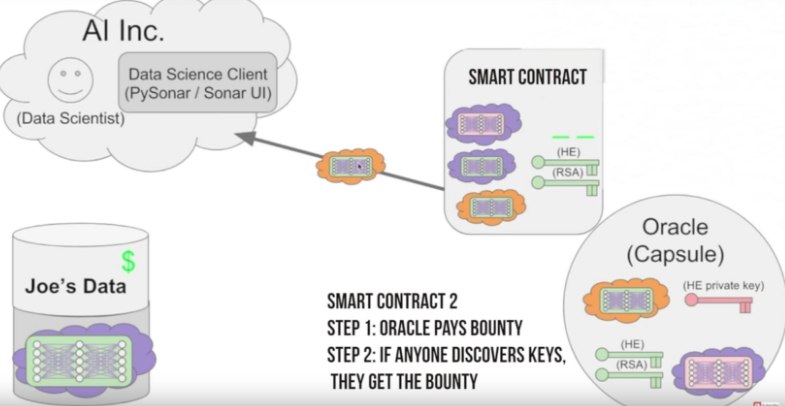
\includegraphics[width=0.90\columnwidth]{blockchain-oracle.jpg}
\caption{Smart contracts and oracles}
\end{figure}

\end{frame}

% =================================================================
\section{Machine Learning \& AI}
% -----------------------------------------------------------------
\begin{frame}[allowframebreaks]
\frametitle{\insertsection}

\begin{itemize}
\item People and companies that make use of machine learning need access to large datasets in order to train their models. On the other hand, it is \linebreak difficult for dataset owners to rent their data. 
\begin{itemize}
\item \Eg we would like to access FaceBook's data to train facial recognition software, but FB does not trust anybody outside its organization. 
\item Blockchain applications such as OpenMined allow machine learning experts and dataset owners to trust each other by making use of oracles. 
\end{itemize}
\item In the near future, blockchains could also be used to incentivize drivers to share their data by providing a mechanism to pay for their data. This will be extremely useful for developing self-driving cars. 
\begin{itemize}
\item \Eg BigchainDB (Toyota), DOVU (Jaguar + Land Rover). 
\end{itemize}
\end{itemize}

\end{frame}

% =================================================================
\section{Health Care}
% -----------------------------------------------------------------
\begin{frame}[allowframebreaks]
\frametitle{\insertsection}

\begin{itemize}
\item Most hospitals lack a secure platform to store and share data, and they are prone to attack by hackers because of the sensitivity of medical records. 
\item By implementing blockchain-based record management systems, hospitals can ensure patients data is accessible only to them and to their caring physicians.
\item In addition to being private, these systems are tamper-proof, meaning that records are impossible to falsify.
\item Two startups in this industry are Gem and Tierion. 

\end{itemize}

\end{frame}

% =================================================================
\section{NGOs and Government}
% -----------------------------------------------------------------
\begin{frame}[allowframebreaks]
\frametitle{\insertsection}

\begin{itemize}
\item The most common problems in these sectors are lack of transparency, inefficiency, and corruption. Therefore charities and NGOs that could allow their benefactors to track their donations are likely to gain competitive advantage over their peer institutions. 
\begin{itemize}
\item \Eg blockchain-based charity like BitGive takes advantage of the distributed ledger architecture of its system to let donors verify that their contributions reach their intended party. 
\end{itemize}
\item Distribution of public benefits \emph{(welfare)} is another activity that could be improved by the blockchain. \Eg startup GovCoin in the UK. 
\item In general, blockchain in government could lead to improved transparency and efficiency of operations. \Eg Dubai is aiming to migrate all of its documents to the blockchain-based system CONSENSYS by 2020. 
\end{itemize}

\end{frame}

% =================================================================
\section{Other Industries}
% -----------------------------------------------------------------
\begin{frame}[allowframebreaks]
\frametitle{\insertsection}

\begin{itemize}
\item Retail: 
\begin{itemize}
\item OpenBazaar, OB1
\end{itemize}
\item Real Estate: 
\begin{itemize}
\item Ubitquity
\end{itemize}
\item Entertainment (music): 
\begin{itemize}
\item MyCelia, ujo Music
\end{itemize}
\end{itemize}

\end{frame}

\end{document}
